\documentclass{jsarticle}
\usepackage{graphicx}

\begin{document}
\section{目的}
    今回は, ~総務省, ~内閣府から公開されている統計データから,
    ~各都道府県間の情報格差について調べた.

    対象として, ~私たちが住む新潟の他に, ~大阪, ~山口, ~福岡,
    ~福島, ~長野, ~秋田, ~岐阜を選んだ.
    ~これらの都道府県は, ~班のメンバーのゆかりの地の他,
    ~新潟に面積が近い都道府県を選んだ.

\section{方法}
    調査方法として, ~主に授業内で配布されてデータを使用した.
    ~各県のブロードバンド接続率が情報格差に繋がっていると考え,
    ~様々なパラメータと比較をし, ~視覚化をした.
    ~主にメンバー全員でデータを調査し, ~まとめた.

    また, ~今回は全て平成26年度のデータを使用した.

\section{結果}
    以下に調査結果を示す.

    \subsection{所得と接続率}
        \begin{center}
            \begin{figure}
                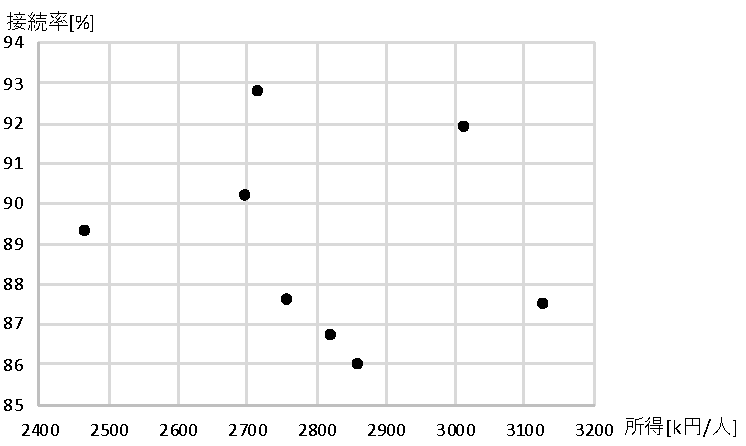
\includegraphics[width=6cm]{所得.pdf}
                \caption{所得-接続率散布図}
                \label{fig:所得}
            \end{figure}
        \end{center}
        

    \subsection{所得増加率と接続率}

    \subsection{人口と接続率}

    \subsection{人口増加率と接続率}

    \subsection{人口密度と接続率}
        配布資料に書かれてない情報として,
        ~各県の人口密度を調査してみた.

        これは, ~人口密度が高い都道府県,
        ~所謂都会に近い場所の方が接続率が高いと考えたからである.

\section{考察 $\cdot$ 感想}
    各調査を通して, ~各項目と接続率とにはあまり関係性がみられないことがわかった.


%\begin{thebibliography}
%    \bibitem{プリント} 2019-Ec3計算機システム資料(5)
%\end{thebibliography}
\end{document}